\chapter{Volumenkontrol}
\label{volumenkontrol}

\section{Design}
\label{volumenkontrol-design}

\begin{figure}[h]
\centering
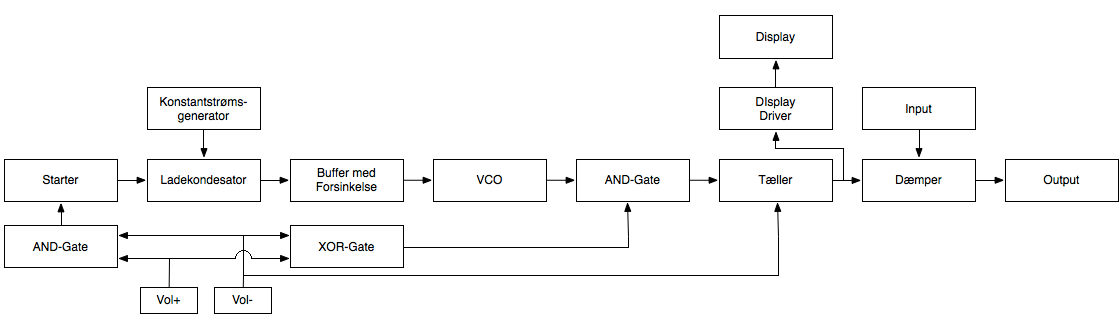
\includegraphics[width=\textwidth]{teknisk/volumenkontrol/blokdiagram.png}
\caption{Blokdiagram over volumenkontrollen}
\label{fig:volumenkontrol_opbygning}
\end{figure}

\section{Simulering}
\label{volumenkontrol-simulering}

\begin{figure}[h]
\centering
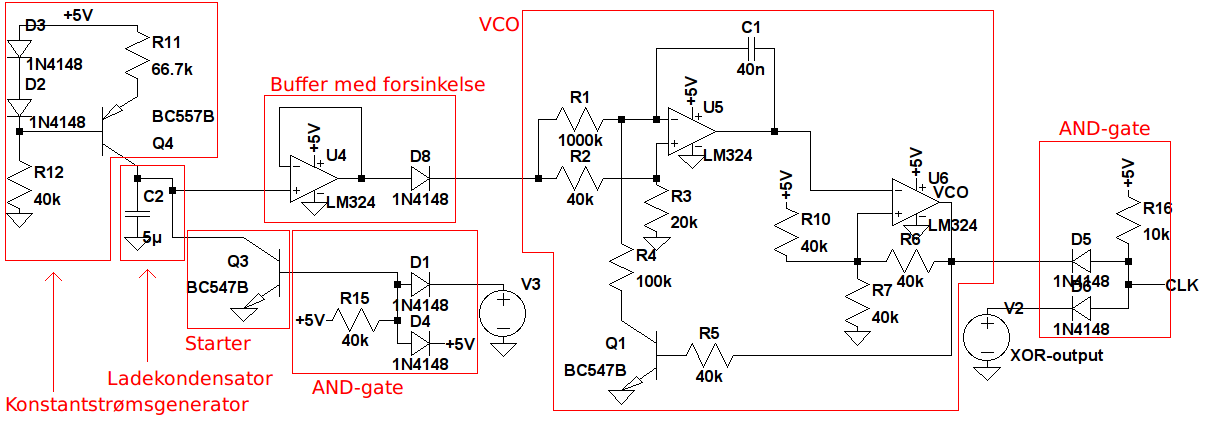
\includegraphics[width=\textwidth]{teknisk/volumenkontrol/diagram.png}
\caption{Diagram over volumenkontrollen}
\label{fig:volumenkontrol_diagram}
\end{figure}

\subsection{Konstantstrømsgenerator}
\label{volumenkontrol-simulering-konstantstroemsgenerator}

Konstantstrømsgeneratorens opgave er at leve en konstant strøm, denne strøm bruges til at oplade en kondensator (ladekondensatoren). Når en kondensator lades med en konstant strøm, vil spændingen over den stige lineært, dette fremgår også af ligning \ref{equ:konstantstroemsgenerator1}.

\begin{equation}
\label{equ:konstantstroemsgenerator1}
V = \frac{I \cdot t}{C}
\end{equation}

Konstantstrømsgeneratoren er designet med udgangs på at der vil være et spændingsfald på $0,5 V$ over $D_2$, $D_3$, $R_{11}$ og $Q_{4_{BE}}$. I databladet for 1N4148 fremgår det at den vil have en $V_D$ spændingen på $0,5 V$ ved en $I_F$ strøm på $0,1 mA$. Modstanden $R_{12}$ er således givet ved ligningen \ref{equ:konstantstroemsgenerator2}.

\begin{equation}
\label{equ:konstantstroemsgenerator2}
R_{12} = \frac{V_{CC} - 2 \cdot V_D}{I_F} = \frac{5V - 2 \cdot 0,5 V}{0,1 mA} = 40 k\ohm
\end{equation}

Den kondensator som konstantstrømsgeneratoren kaldes ladekondensatoren, denne har en kapacitet på $5 \mu F$ og den ønskede oplade tid er $3 s$. Kondensatoren oplades fra 0 V til $V_{CC} - V_F = 4,5 V$, hvor $V_F$ er spændingen over én diode. Udfra disse to ting kan den konstante strøm, $I_{konst}$, nu beregnes, se ligning \ref{equ:konstantstroemsgenerator3}.

\begin{equation}
\label{equ:konstantstroemsgenerator3}
V_{CC} - V_D = \frac{I_{konst} \cdot t}{C} \Rightarrow 4,5 V = \frac{I_{konst} \cdot 3 s}{5 \mu F} \Rightarrow I_{konst} = 7,5 \mu A
\end{equation}

Spændingen over $R_{11}$ er, som tidligere nævnt, $0,5 V$ og strømmen igennem den er $I_{konst}$, der kan Ohms lov bruges til at beregne modstanden, se ligning \ref{equ:konstantstroemsgenerator4}.

\begin{equation}
\label{equ:konstantstroemsgenerator4}
V_D = R \cdot I_{konst} \Rightarrow 0,5 V = R \cdot 7,5 \mu A \Rightarrow R = 66,7 k\ohm
\end{equation}

\subsection{Starter}
\label{volumenkontrol-simulering-starter}

Starterens opgave er at holde spændingen over ladekondensatoren på $0 V$, når der ikke trykkes på en af volumenknapperne. Dette gøres ved at lede al den strøm som konstantstrømsgeneratoren levere til stel. Dette gøres for at sikre at ladekondensatoren er klar til at starte opladningen lige når der trykkes på en af volumenknapperne.

\subsection{Buffer med forsinkelse}
\label{volumenkontrol-simulering-buffer}

Bufferen sikre at ladekondensatoren bliver lineært opladet, dette gøres ved ikke at belaste konstantstrømsgeneratoren eller ladekondensatoren. Forsinkelsen laves ved hjælp af en diode. Dioden forsinker signalet ved blot at have et spændingsfald over den, det betyder at spændingen først skal vokse op, før der kommer en kontrolspænding til VCO'en.

\subsection{VCO}
\label{volumenkontrol-simulering-vco}

En VCO, Voltage Controlled Oscillator, levere et konstant signal hvor frekvensen er afhængig af en kontrolspænding. Der er taget udgangspunkt i en VCO fra databladet for en LM324. VCO'en kan deles op i to blokke en integrator og en schmidt-trigger. Det er udgangen fra schmidt-triggeren der bestemmer hvilken af de to spændinger integrator arbejder udfra.

\subsection{Tæller}
\label{volumenkontrol-simulering-taeller}

Det er tællerens opgave at holde styr på hvad volumenniveauet er. Der tælles op eller ned når der trykkes på én af de to volumenknapper. Hvor hurtigt der skal tælles bestemmes af det AND'ende signal fra VCO'en og XOR-gaten. Tælleren danner også grundlag for hvad der skal stå i displayet.

\subsection{Display driver}
\label{volumenkontrol-simulering-display_driver}

Display driveren konvertere signalet fra tælleren til et signal der kan vises på de to 7-segment displays. Display driveren er opbygget af digitale gates, dette er gjort for at få flere forskellige slags kredsløb i HiFi-forstærkeren.

\subsection{Display}
\label{volumenkontrol-simulering-display}



\subsection{Summations forstærker}
\label{volumenkontrol-simulering-summations_forstaerker}



\subsection{Dæmper}
\label{volumenkontrol-simulering-daemper}



\section{Accepttest}
\label{volumenkontrol-accepttest}

